A NASNet iteratív tanításának eredményei négy lépésben először 1000 majd 5000 azután 10000 végül pedig 25000 képes halmazon. Ezelet a lépéseket 1k, 5k 10k 25k rövidítésekkel fogom jelölni.
A NASNet esetében 5-5-3-2 Epoch tanítás történt a rendszer kiemelkedően magas futási ideje miatt.

%1K-----------------------------------------------------------------------------
\subsubsection{1k adathalmazon történő tanítás lépései NASNet modellen.}
  \begin{itemize} 
    \item Epoch 1/5 - train: 228/228 [00:46<00:00,4.94it/s]
    \item Epoch 1/5 - val: 282/282 [01:21<00:00,3.47it/s]
    \item Epoch 1: Train loss=4.4943, acc=0.0789 Val loss=3.2968, acc=0.2334
    \item Epoch 2/5 - train: 228/228 [00:44<00:00,5.10it/s]
    \item Epoch 2/5 - val: 282/282 [01:21<00:00,3.47it/s]
    \item Epoch 2: Train loss=2.5769, acc=0.3640 Val loss=3.0409, acc=0.3142
    \item Epoch 3/5 - train: 228/228 [00:45<00:00,5.03it/s]
    \item Epoch 3/5 - val: 282/282 [01:21<00:00,3.47it/s]
    \item Epoch 3: Train loss=1.2119, acc=0.6985 Val loss=3.3285, acc=0.3500
    \item Epoch 4/5 - train: 228/228 [00:44<00:00,5.07it/s]
    \item Epoch 4/5 - val: 282/282 [01:21<00:00,3.47it/s]
    \item Epoch 4: Train loss=0.4945, acc=0.8761 Val loss=4.1111, acc=0.3110
    \item Epoch 5/5 - train: 228/228 [00:44<00:00,5.07it/s]
    \item Epoch 5/5 - val: 282/282 [01:21<00:00,3.47it/s]
    \item Epoch 5: Train loss=0.2662, acc=0.9441 Val loss=4.0139, acc=0.3285
  \end{itemize}

\subsubsection{1k adathalmazon történő tanítás grafikonja NASNet modellen.}
  \begin{figure}[H]
    \centering
    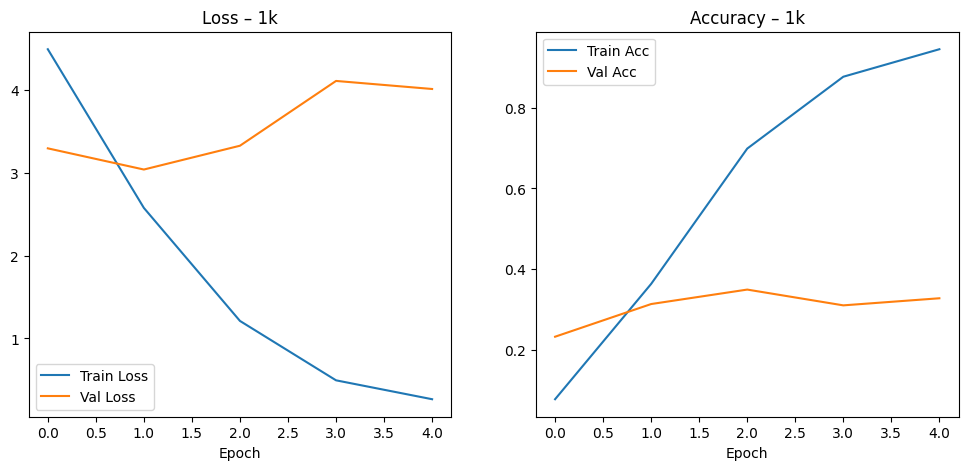
\includegraphics[width=1.0\textwidth]{images/phase03/phase03_NASNet_1K_learning_curve.png}
    \caption{1k adathalmazon történő tanítás grafikonja NASNet modellen.}
    \label{fig:phase03_NASNet_1K_learning_curve}
  \end{figure}

  \subsubsection{1k adathalmazon történő tanítás eredményei.}
    \begin{center}
      \begin{longtable}{l c}
      \caption{1k tanítás NASNet-en.} \label{tab:phase03_NASNet_1k} \\
      \toprule
      \textbf{Metrika} & \textbf{Érték} \\
      \midrule
      \endfirsthead
      \toprule
      \textbf{Metrika} & \textbf{Érték} \\
      \midrule
      \endhead
      Top-1 Accuracy & 0.3324 \\
      Top-5 Accuracy & 0.6131 \\
      Precision      & 0.3456 \\
      Recall         & 0.3690 \\
      F1-score       & 0.3261 \\
      Inference time & 81.04 sec \\
      \bottomrule
      \end{longtable}
    \end{center}

%5K-----------------------------------------------------------------------------
\subsubsection{5k adathalmazon történő tanítás lépései NASNet modellen.}
  \begin{itemize} 
    \item Epoch 1/5 - train: 1226/1226 [04:01<00:00, 5.09it/s]
    \item Epoch 1/5 - val: 282/282 [01:21<00:00, 3.47it/s]
    \item Epoch 1: Train loss=3.1256, acc=0.2678 Val loss=3.1782, acc=0.3521
    \item Epoch 2/5 - train: 1226/1226 [04:02<00:00, 5.06it/s]
    \item Epoch 2/5 - val: 282/282 [01:21<00:00, 3.47it/s]
    \item Epoch 2: Train loss=1.7259, acc=0.5279 Val loss=2.9296, acc=0.4284
    \item Epoch 3/5 - train: 1226/1226 [04:00<00:00, 5.09it/s]
    \item Epoch 3/5 - val: 282/282 [01:21<00:00, 3.47it/s]
    \item Epoch 3: Train loss=0.9826, acc=0.7189 Val loss=3.2216, acc=0.4299
    \item Epoch 4/5 - train: 1226/1226 [04:00<00:00, 5.09it/s]
    \item Epoch 4/5 - val: 282/282 [01:21<00:00, 3.47it/s]
    \item Epoch 4: Train loss=0.5718, acc=0.8427 Val loss=3.8691, acc=0.3981
    \item Epoch 5/5 - train: 1226/1226 [04:02<00:00, 5.06it/s]
    \item Epoch 5/5 - val: 282/282 [01:21<00:00, 3.47it/s]
    \item Epoch 5: Train loss=0.4060, acc=0.8800 Val loss=4.6202, acc=0.4074
  \end{itemize}

\subsubsection{5k adathalmazon történő tanítás grafikonja NASNet modellen.}
  \begin{figure}[H]
    \centering
    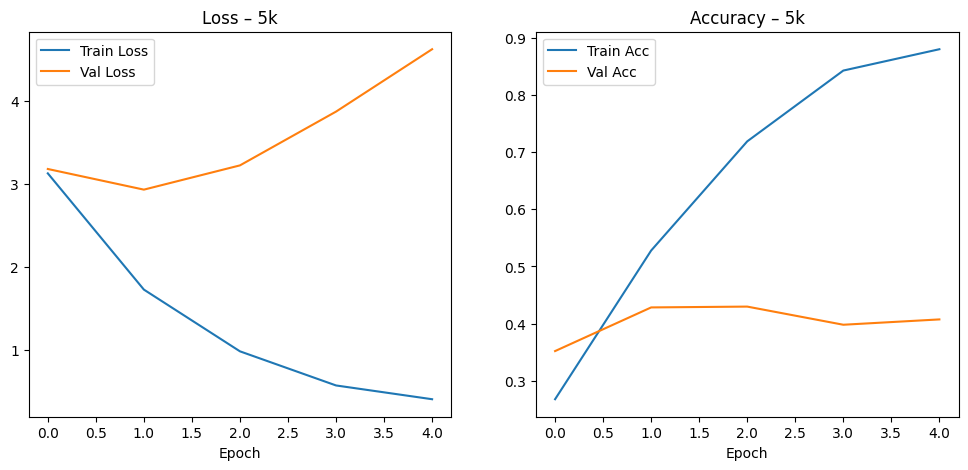
\includegraphics[width=1.0\textwidth]{images/phase03/phase03_NASNet_5K_learning_curve.png}
    \caption{5k adathalmazon történő tanítás grafikonja NASNet modellen.}
    \label{fig:phase03_NASNet_5K_learning_curve}
  \end{figure}

\subsubsection{5k adathalmazon történő tanítás eredményei.}
  \begin{center}
    \begin{longtable}{l c}
    \caption{5k tanítás NASNet-en.} \label{tab:phase03_NASNet_5k} \\
    \toprule
    \textbf{Metrika} & \textbf{Érték} \\
    \midrule
    \endfirsthead
    \toprule
    \textbf{Metrika} & \textbf{Érték} \\
    \midrule
    \endhead
    Top-1 Accuracy & 0.4062 \\
    Top-5 Accuracy & 0.6912 \\
    Precision      & 0.4096 \\
    Recall         & 0.4284 \\
    F1-score       & 0.3844 \\
    Inference time & 81.54 sec \\
    \bottomrule
    \end{longtable}
  \end{center}

%10K-----------------------------------------------------------------------------
\subsubsection{10k adathalmazon történő tanítás lépései NASNet modellen.}
  \begin{itemize} 
    \item Epoch 1/3 - train: 2480/2480 [08:11<00:00, 5.05it/s]
    \item Epoch 1/3 - val: 282/282 [01:21<00:00, 3.46it/s]
    \item Epoch 1: Train loss=2.7872, acc=0.3202 Val loss=3.1433, acc=0.4165
    \item Epoch 2/3 - train: 2480/2480 [08:13<00:00, 5.03it/s]
    \item Epoch 2/3 - val: 282/282 [01:21<00:00, 3.46it/s]
    \item Epoch 2: Train loss=1.6655, acc=0.5420 Val loss=2.9456, acc=0.4947
    \item Epoch 3/3 - train: 2480/2480 [08:13<00:00, 5.02it/s]
    \item Epoch 3/3 - val: 282/282 [01:21<00:00, 3.46it/s]
    \item Epoch 3: Train loss=1.0698, acc=0.6930 Val loss=3.4763, acc=0.4495
  \end{itemize}

\subsubsection{10k adathalmazon történő tanítás grafikonja NASNet modellen.}
  \begin{figure}[H]
    \centering
    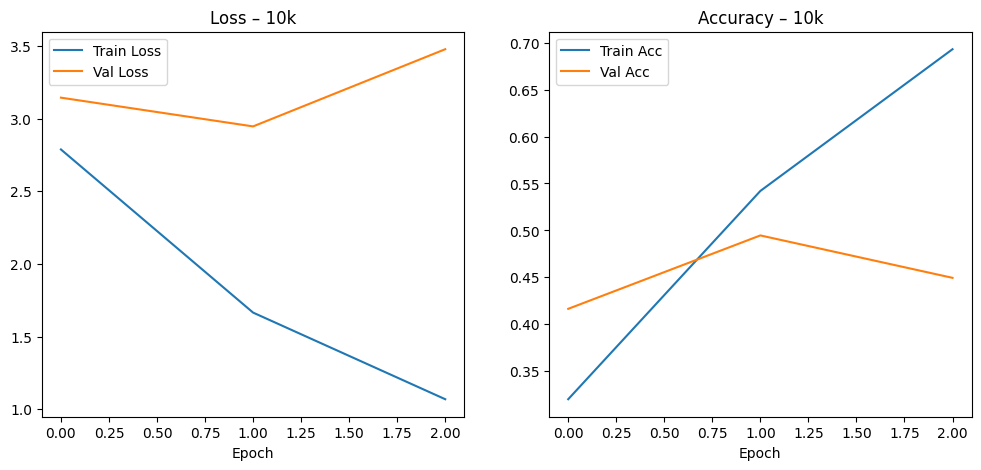
\includegraphics[width=1.0\textwidth]{images/phase03/phase03_NASNet_10K_learning_curve.png}
    \caption{10k adathalmazon történő tanítás grafikonja NASNet modellen.}
    \label{fig:phase03_NASNet_10K_learning_curve}
  \end{figure}

\subsubsection{10k adathalmazon történő tanítás eredményei.}
  \begin{center}
    \begin{longtable}{l c}
    \caption{10k tanítás NASNet-en.} \label{tab:phase03_NASNet_10k} \\
    \toprule
    \textbf{Metrika} & \textbf{Érték} \\
    \midrule
    \endfirsthead
    \toprule
    \textbf{Metrika} & \textbf{Érték} \\
    \midrule
    \endhead
    Top-1 Accuracy & 0.4438 \\
    Top-5 Accuracy & 0.7665 \\
    Precision      & 0.4252 \\
    Recall         & 0.4736 \\
    F1-score       & 0.4133 \\
    Inference time & 81.46 sec \\
    \bottomrule
    \end{longtable}
  \end{center}

%25K-----------------------------------------------------------------------------
\subsubsection{25k adathalmazon történő tanítás lépései NASNet modellen.}
  \begin{itemize} 
    \item Epoch 1/2 - train: 6242/6242 [20:45<00:00, 5.01it/s]
    \item Epoch 1/2 - val: 282/282 [01:21<00:00, 3.46it/s]
    \item Epoch 1: Train loss=2.4012, acc=0.3956 Val loss=2.6687, acc=0.4672
    \item Epoch 2/2 - train: 6242/6242 [20:43<00:00, 5.02it/s]
    \item Epoch 2/2 - val: 282/282 [01:21<00:00, 3.46it/s]
    \item Epoch 2: Train loss=1.5766, acc=0.5719 Val loss=2.7290, acc=0.4751
  \end{itemize}

\subsubsection{25k adathalmazon történő tanítás grafikonja NASNet modellen.}
  \begin{figure}[H]
    \centering
    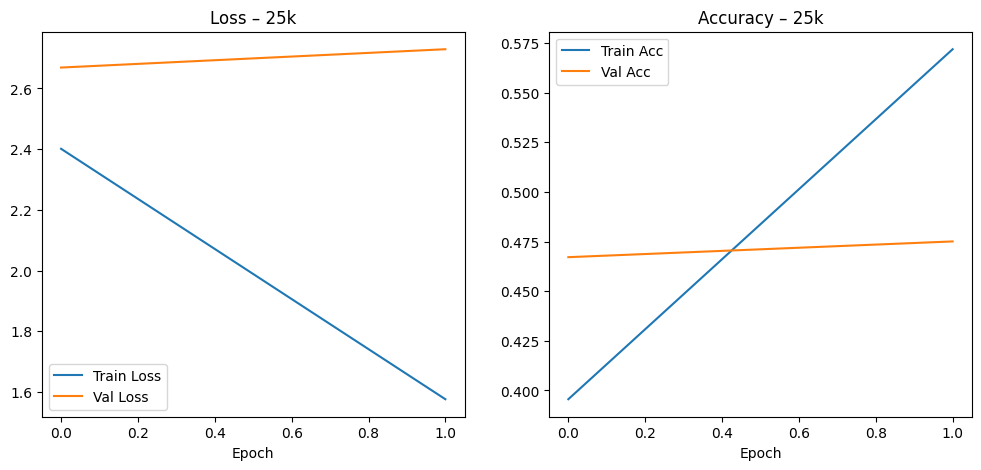
\includegraphics[width=1.0\textwidth]{images/phase03/phase03_NASNet_25K_learning_curve.png}
    \caption{25k adathalmazon történő tanítás grafikonja NASNet modellen.}
    \label{fig:phase03_NASNet_25K_learning_curve}
  \end{figure}

\subsubsection{25k adathalmazon történő tanítás eredményei.}
  \begin{center}
    \begin{longtable}{l c}
    \caption{25k tanítás NASNet-en.} \label{tab:phase03_NASNet_25k} \\
    \toprule
    \textbf{Metrika} & \textbf{Érték} \\
    \midrule
    \endfirsthead
    \toprule
    \textbf{Metrika} & \textbf{Érték} \\
    \midrule
    \endhead
    Top-1 Accuracy & 0.4750 \\
    Top-5 Accuracy & 0.8059 \\
    Precision      & 0.4812 \\
    Recall         & 0.5289 \\
    F1-score       & 0.4688 \\
    Inference time & 81.43 sec \\
    \bottomrule
    \end{longtable}
  \end{center}

\subsubsection{NASNet iteratív tanítás összefoglaló}
  \begin{center}
    \begin{longtable}{lllllll}
    \caption{Összehasonlító táblázat a NASNet iteratív tanításáról.}\label{tab:phase3_NASNet_summary_table}\\
    \toprule
    Minta & Top-1 & Top-5 & Precision & Recall & F1 & Time(s) \\
    \midrule
    \endfirsthead
    \toprule
    Minta & Top-1 & Top-5 & Precision & Recall & F1 & Time(s) \\
    \midrule
    \endhead
    1k & 0.3324 & 0.6131 & 0.3456 & 0.3690 & 0.3261 & 81.04 \\
    5k & 0.4062 & 0.6912 & 0.4096 & 0.4284 & 0.3844 & 81.54 \\
    10k & 0.4438 & 0.7665 & 0.4252 & 0.4736 & 0.4133 & 81.46 \\
    25k & 0.4750 & 0.8059 & 0.4812 & 0.5289 & 0.4688 & 81.43 \\
    \bottomrule
    \end{longtable}
  \end{center}
  
  \subsubsection{Összehasonlító grafikon a NASNet iteratív tanításáról.}
  \begin{figure}[H]
    \centering
    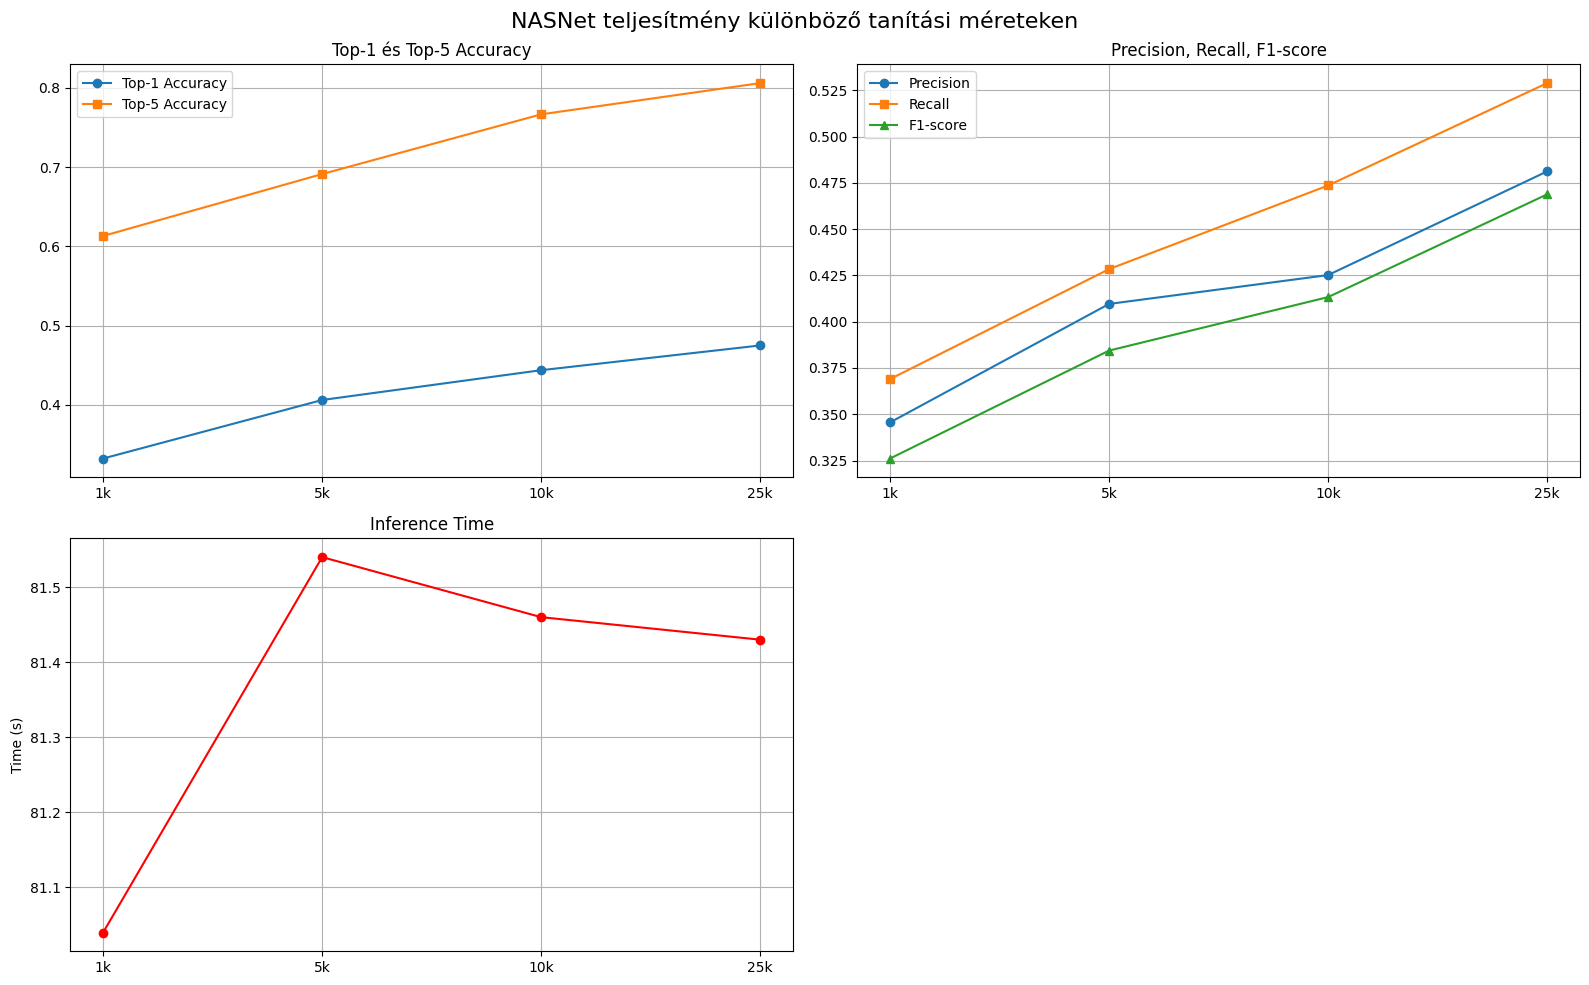
\includegraphics[width=1.0\textwidth]{images/phase03/phase03_NASNet_summary_curve.png}
    \caption{Összehasonlító grafikon a NASNet iteratív tanításáról.}
    \label{fig:phase03_NASNet_summary_curve}
  \end{figure}

  \subsubsection{Összehasonlító metrika grafikon a NASNet iteratív tanításáról.}
  \begin{figure}[H]
    \centering
    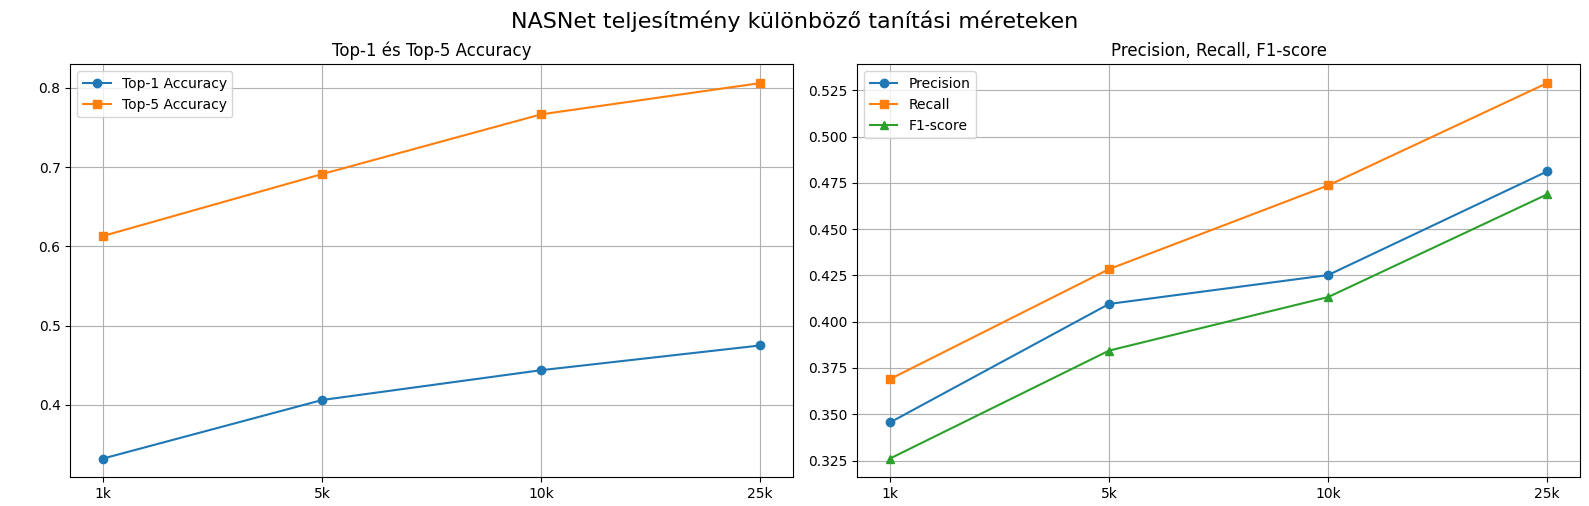
\includegraphics[width=1.0\textwidth]{images/phase03/phase03_NASNet_summary_curve_metrics.png}
    \caption{Összehasonlító metrika grafikon a NASNet iteratív tanításáról.}
    \label{fig:phase03_NASNet_summary_curve_metrics}
  \end{figure}

  \subsubsection{Összehasonlító idő grafikon a NASNet iteratív tanításáról.}
  \begin{figure}[H]
    \centering
    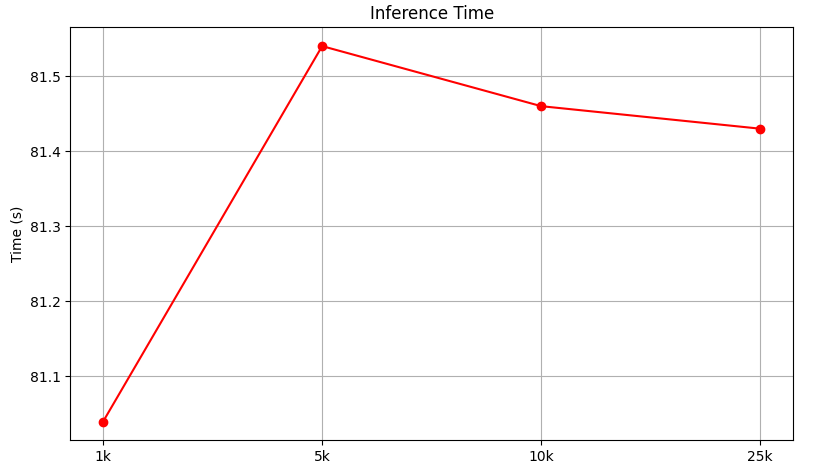
\includegraphics[width=1.0\textwidth]{images/phase03/phase03_NASNet_summary_curve_time.png}
    \caption{Összehasonlító idő grafikon a NASNet iteratív tanításáról.}
    \label{fig:phase03_NASNet_summary_curve_time}
  \end{figure}

  \subsubsection{Összehasonlító grafikon a NASNet iteratív tanításáról 10 EPOCH-on keresztül.}
  \begin{figure}[H]
    \centering
    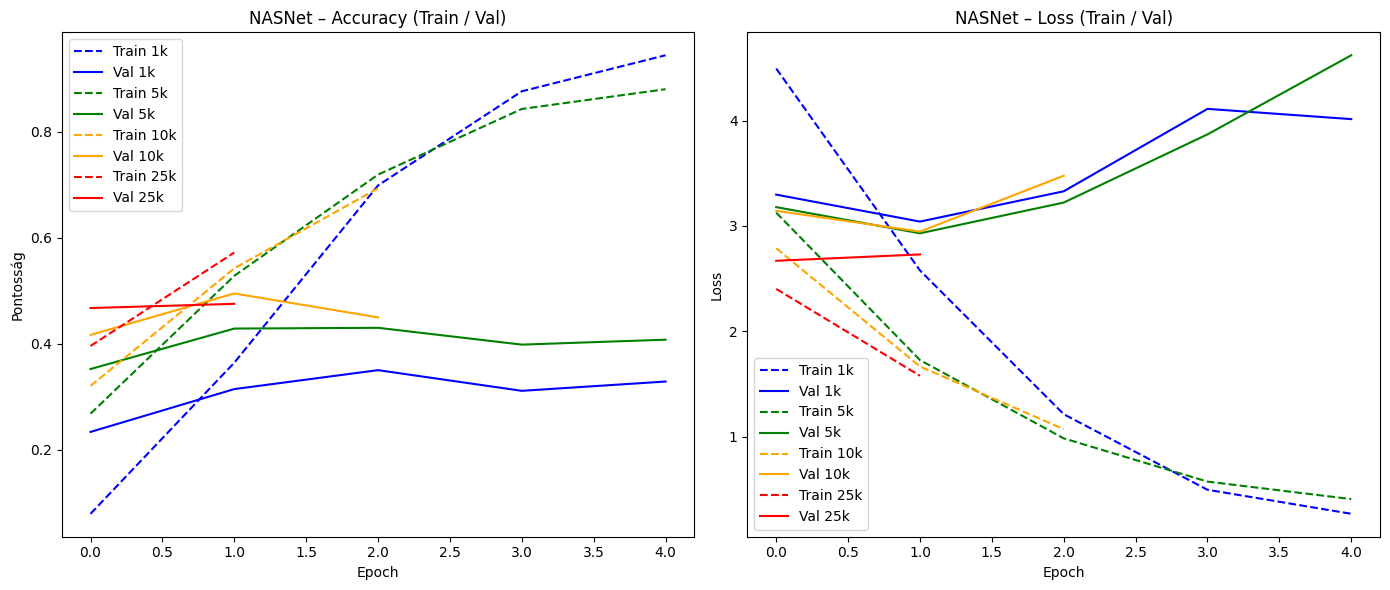
\includegraphics[width=1.0\textwidth]{images/phase03/phase03_NASNet_learning_summary_curve.png}
    \caption{Összehasonlító grafikon a NASNet iteratív tanításáról 10 EPOCH-on keresztül.}
    \label{fig:phase03_NASNet_learning_summary_curve}
  \end{figure}

  \subsubsection{Összehasonlító Confusion Matrix a NASNet iteratív tanításáról.}
  \begin{figure}[H]
    \centering
    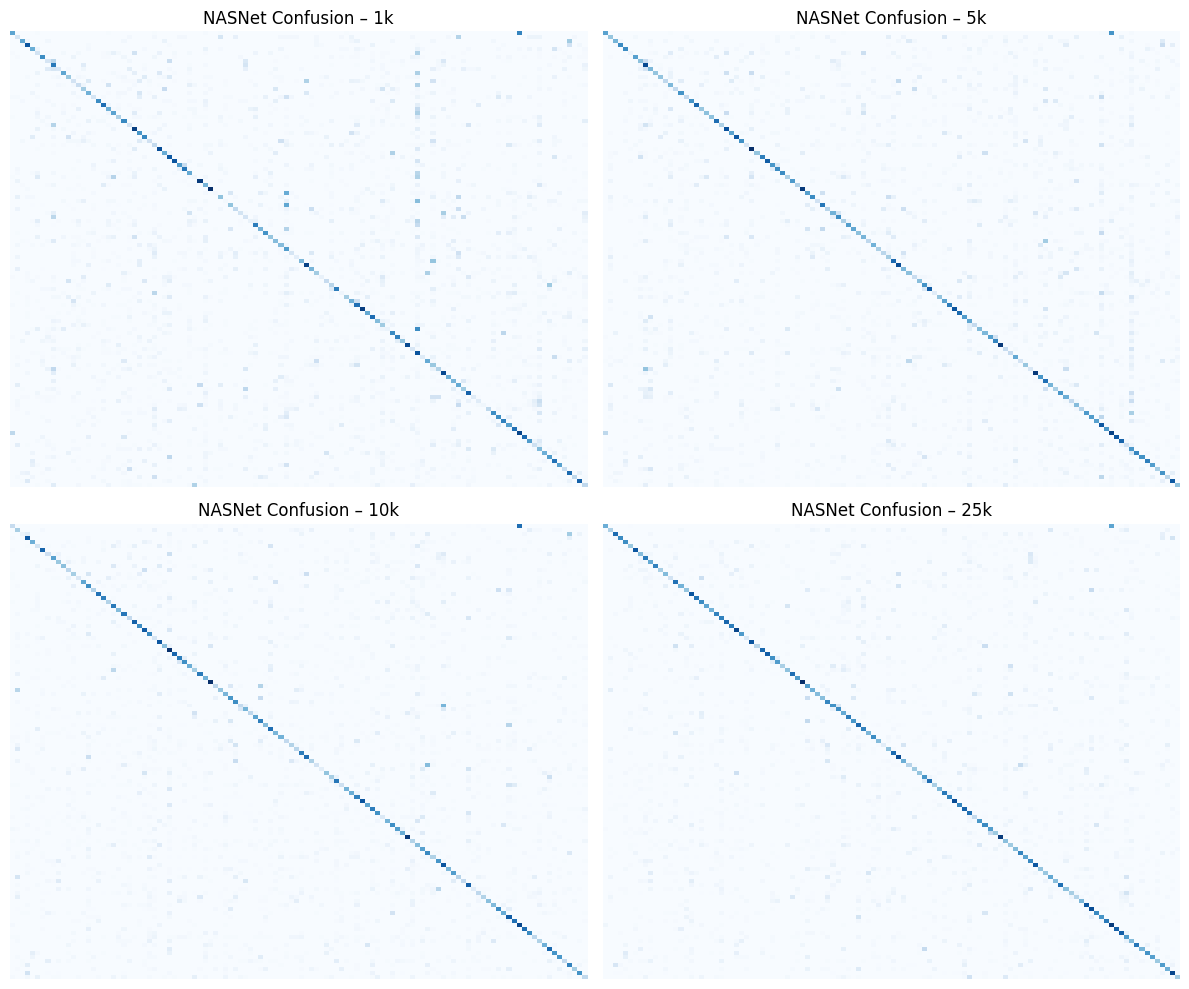
\includegraphics[width=1.0\textwidth]{images/phase03/phase03_NASNet_Confusion_Matrix_summary_curve.png}
    \caption{Összehasonlító Confusion Matrix a NASNet iteratív tanításáról 10 EPOCH-on keresztül.}
    \label{fig:phase03_NASNet_Confusion_Matrix_summary_curve}
  \end{figure}